\begin{frame}[fragile,t]{Metodologia de Trabalho}
	\begin{figure}[h!]
		\centering
		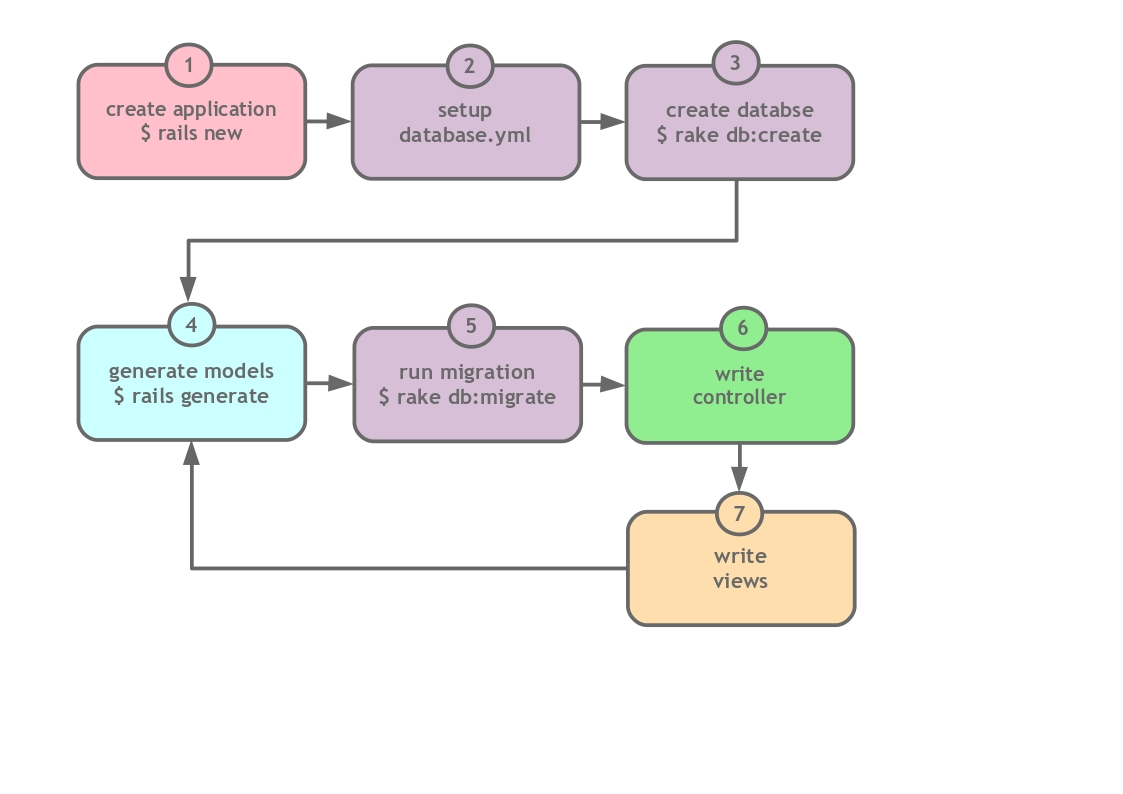
\includegraphics[width=.9\textwidth]{imagens/metodologia-de-trabalho.jpg}
	\end{figure}
\end{frame}

\begin{frame}[allowframebreaks, fragile,t]{Passos Iniciais do Blog App}
	\begin{enumerate}
	    \item Inicie uma janela de terminal e digite no prompt:
	     \begin{lstlisting}[style=BashInputBasicStyle]
		     $ cd 
		     $ rails new blog
	     \end{lstlisting}
%	    \item Utilize o gerador \verb|scaffold| para criar os 
%	    componentes MVC para as postagens e os comentários
%	     \begin{lstlisting}[style=BashInputBasicStyle]
%					$ rails generate scaffold post \ 
%			     title:string body:text
%					$ rails generate scaffold comment post_id:integer \
%					 body:text
%	     \end{lstlisting}
%	    \item Gere as tabelas \verb|post| e \verb|comment| no banco de dados
%	    \begin{lstlisting}[style=BashInputBasicStyle]
%		    $ rake db:migrate
%	    \end{lstlisting}
%	    
%	    \item Visualize todas as URLs reconhecidas pela sua aplicação digitando:
%	    \begin{lstlisting}[style=BashInputBasicStyle]
%	    $ rake routes
%	    \end{lstlisting}
	     \item Inicie o servidor web embutido:
	     \begin{lstlisting}[style=BashInputBasicStyle]
	     $ rails s
	     \end{lstlisting}
	     
	     \item Abra uma janela do navegador e digite:
	     \begin{lstlisting}[style=BashInputBasicStyle]
	     $ http://localhost:3000
	     \end{lstlisting}
	\end{enumerate}
  
\end{frame}
